\section{Publish Subscribe}
% Deisgn Pattern : Event driven messaging 
\begin{patdescription}

\item[Traceability]
The notification mechanism of the Docker Registry uses the Publish Subscribe Pattern \cite{docknotif}.

\item[Source]
Pattern Oriented Software Architecture- Volume 1
%http://soapatterns.org/designpatterns/eventdrivenmessaging

\item[Issue] The user wants to be alerted about certain events/changes that occur in a registry.
The notification system needs a mechanism in order to send those events to the user.

\item[Assumptions/Constraints] 
This pattern is used at a lower level in the Docker Registry/Active Repository Pattern.



\item[Solution]

\item[Rationale] 

%TODO fix, remove the big quote. Use POSA or something

\begin{quote}
"Notifications are sent to endpoints via HTTP requests. Each configured endpoint has isolated queues, retry configuration and http targets within each instance of a registry. When an action happens within the registry, it is converted into an event which is dropped into an inmemory queue. When the event reaches the end of the queue, an http request is made to the endpoint until the request succeeds. The events are sent serially to each endpoint but order is not guaranteed."% it seems like it's the way it works
\end{quote} 

\item[Implications] %After the integration of the Publish-Suscribe pattern BLABLABLA
The Publish Suscribe Pattern enhances Integrability,Modifiability because publisher and suscribers aren't directly connected.% develop

\item [Related Patterns]
Shared/Active Repository Pattern


\end{patdescription}

\begin{figure}[H]
\centering
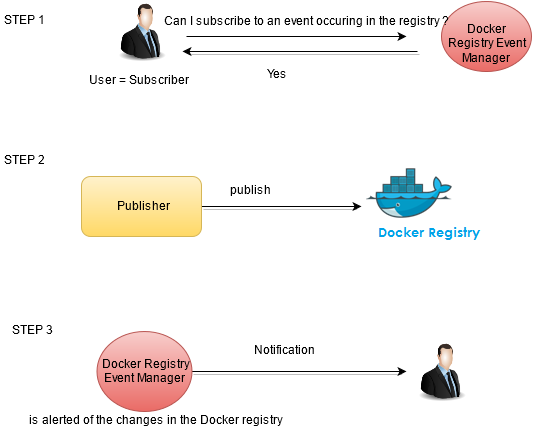
\includegraphics[scale=0.7]{5-patterns/images/RegistryPS.png}
\caption{Events managing- Publish Subscribe Pattern}
\label{fig:publish-subscribe}
\end{figure}

